\documentclass[border=1cm]{standalone}
\usepackage{amsmath}

\usepackage{tikz}
\usetikzlibrary{shapes,arrows,fit,automata}
\usetikzlibrary{positioning}


\begin{document}

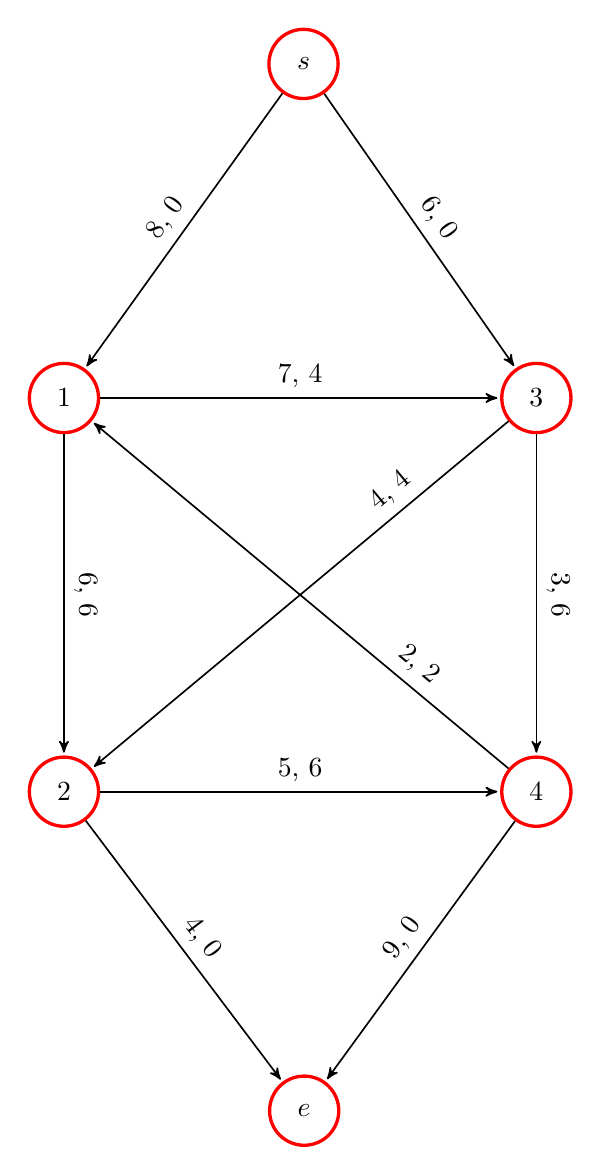
\begin{tikzpicture}[->,>=stealth',shorten >=1pt,auto,node distance=6cm,
    semithick]
\tikzstyle{every state}=[circle, black, draw=red, very thick]

\node[state]          (1)                         {$1$};

\node[state]         (2) [below of=1,yshift=1cm]  {$2$};
\node[state]         (3) [right of=1]             {$3$};
\node[state]         (4) [below of=3,yshift=1cm]  {$4$};

\node[state]         (s) [above right of=1, xshift=-1.2cm]  {$s$};
\node[state]         (e) [below right =3.4cm and 2.4cm of 2] {$e$};



\path   (1) edge node [sloped,above]            {6, 6}  (2)
        (4) edge node[sloped,above,near start]  {2, 2}  (1)
        (1) edge node[sloped,above]             {7, 4}  (3)
                                                

        (2) edge node[sloped,above ]            {5, 6}  (4)
        
        (3) edge node[sloped,above,near start]  {4, 4}  (2)                       
        (3) edge node [sloped,above]            {3, 6}  (4)

        (s) edge            node[sloped,above]  {8, 0} (1)
        (s) edge            node[sloped,above]  {6, 0} (3)
        (2) edge            node[sloped,above]  {4, 0} (e)
        (4) edge            node[sloped,above]  {9, 0} (e);
        
\end{tikzpicture}
\end{document}